\documentclass{article}

\usepackage{tikz}
\usetikzlibrary{shapes.misc}


\title{Chapter 2.4 Exercise Solutions}
\author{Jason Moreau}

\begin{document}

\maketitle
\section*{Conceptual}


\subsection*{Question 1a.}
A flexible statistical learning method would be \textbf{worse} if the sample size \textit{n} is extremely large, and the number of predictors \textit{p} is small because a flexible method requires more variables (parameters) to reduce the errors.

\subsection*{Question 1b.}
A flexible statistical learning method would be \textbf{better} if the number of predictors \textit{p} is extremely large, and the number of observations \textit{n} is small because it would provide a better fit.

\subsection*{Question 1c.}
A flexible statistical learning method would be be \textbf{better} if the predictors and response is highly non-linear because the flexible method would provide a better fit of the observations.

\subsection*{Question 1d.}
A flexible statistical learning method would be \textbf{worse} if the variance of the error terms, i.e. $\sigma^{2}$ = Var($\varepsilon$), is extremely high because it would overfit the model and provide an inaccurate reading for the analyst.

\subsection*{Question 2a.}
This scenario is a regression problem and we are most interested in inference. We are trying to determine the relationship between the dependent and independent variables/predictors. \\
\newline
\textit{n} = 500 firms in the U.S. \newline
\textit{p} = profit, number of employees, industry, and the CEO salary 

\subsection*{Question 2b.}
This scenario is a classification problem and we are most interested in prediction. We are trying to determine whether or not the product will be a \textit{success} or \textit{failure}. \\
\newline
\textit{n} = 20 similar products that were previously launched \newline
\textit{p} = success or failure, price charged, marketing budget, competition price, and ten other variables 

\subsection*{Question 2c.}
This scenario is a regression problem and we are most interested in prediction. We are trying to determine the relationship between the dependent (\% change in the USD/Euro exchange rate) and independent variables. \\
\newline
\textit{n} = Weekly data for all of 2012 \newline
\textit{p} = \% change each week in USD/Euro, the \% change in the US market, the \% change in the British market, and the \% change in the German market

\subsection*{Question 4a.}
\textbf{Classification} \newline
- To find how many dogs vs. cats are in animal shelters in the United States \newline
- To find which Japanese vehicle brand is purchased more often -- Honda or Toyota \newline
- To find which college major is most popular \newline
\textbf{Regression} \newline
- Find relationship between stock prices and bond rates \newline
- Find relationship between life expectancy and income \newline
- Find relationship between engine cylinders and miles per gallon \newline
\textbf{Cluster} \newline
- Find ethnicities within a city \newline
- Find the gender demographic of a university \newline
- Find the income demographic of a town \newline

\subsection*{Question 5}
The advantage of a very flexible (verses a less flexible) approach for regression or classification is that it provides a better
level when conducting prediction modeling. The disadvantage is that level of interpretability suffers and it is not always accurate because it tends to overfit the model.

\subsection*{Question 6}
A parametric approach is that allows the analyst to estimate using a set of parameters (ex. $\beta_{0}$, $\beta_{1}$,
$\beta_{2}$,..$\beta_{p}$). A non-parametric approach attempts to estimate by getting a close a possible to fitting the data. 
An advantage of a parametric approach is that it makes estimating easier because the analyst doesn't have to fit the data the \textit{f}, function of used to estimate the population, Y.  \newline
\begin{center}
Y = \textit{f}(X) + $\epsilon$ 
\end{center}
A disadvantage of a parametric approach is that it might not allow the analyst to pick the right model to obtain the true value of \textit{f}.

\subsection*{Question 7a.}
In the dataset provided we are to make a prediction for Y when X$_{1}$ = X$_{2}$ = X$_{3}$ = 0 using \textit{K}-nearest neighbors. \\ \\
To find the Euclidean distance in two-dimensions when X = 0 we subtract each observation point by zero. \\ \\
\textbf{Observation 1}: \\
(0 - 0) = 0, (3 - 0) = 3, (0 - 0)  = 0 \\ \\
We then square each of the differences to find the absolute value: \\ 
(0)$^{2}$  = 0, (3)$^{2}$ = 9, (0)$^{2}$ = 0 \\ \\
We then find the sum of the squares: 
0 + 9 + 0 = 9 \\ \\
Finally, we take the square root of the sum:
$\sqrt{9}$ = 
% Use this library -tikz to create a circle around final answer
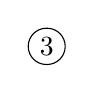
\begin{tikzpicture} [baseline=(char.base)]
\node(char) [draw, shape=rounded rectangle] {3}; 
\end{tikzpicture}
\\ \\
\textbf{Observation 2}: 2 \\
\textbf{Observation 3}: 3.16 \\
\textbf{Observation 4}: 2.23 \\
\textbf{Observation 5}: 1.41 \\
\textbf{Observation 6}: 1.73 \\ 

\subsection*{Question 7b.}
The prediction when \textit{K} = 1 is \textbf{GREEN} because the Observation 5 (1.41) is closest to 1. 

\subsection*{Question 7c.} 
The prediction when \textit{K} = 3 is \textbf{RED} because Observations 2, 5, 6 are closest to each other (take average of Euclidian distance of three observations that are closest to each other and less than 3). Based on probabilities, since Observation 2 and Observation 6 are both Red (\(\frac{2}{3}\)) and Observation 5 is Green (\(\frac{1}{3}\)), KNN will predict \textbf{RED}.
\subsection*{Question 7d.}
If the the Bayes decision boundary in this problem is highly non-linear we expect the best value for \textit{K} to be small. When \textit{K} is small the decision boundary is more non-linear. As \textit{K} grows, the decision boundary becomes more linear.

\end{document}
